\chapter{Results}
\label{chap:results}
\section{Characterization of \emph{M. edulis} hemocyte subpopulations}
The hemolymph of \emph{Mytilus edulis} comprised a mixed population of cells differing in size, morphology and Giemsa staining profiles. Based on these three criteria, the cells could be subdivided into three distinct subpopulations. Staining hemocytes fixed in 5\% formaldehyde or methanol in a 3\% Giemsa solution gave rise to two distinct staining profiles based on the basophilic or eosinophilic nature of their cytoplasmic granules and other various cytoplasmic contents: basophilic and eosinophilic hemocytes. The eosinophilic hemocytes all displayed cytoplasm packed with pink granules of varying size, number and staining intensities. They were of [medium to large size], with a small, round and eccentrically located nucleus i.e., low nuclear:cytoplasmic ratio (n:c ratio). Thus, they are referred to as eosinophilic granulocytes herein. Compared to the eosinophilic granulocytes, basophilic hemocytes were more heterogeneous with respect to cell size, granularity and morphology. They all contained a larger round, oval or bean-shaped nucleus, located centrically or slightly towards one side. But concerning cell size, granularity and n:c ratio, there were essentially two different subpopulations; one population of small lymphocyte-like cells (7 $\pm{x}$ \micro m) displaying a thin a rim of basophilic cytoplasm and no apparent granules, and another population with medium to large cell diameters, displaying abundant basophilic cytoplasm with a few large granules.

[Include a microscope picture displaying all the hemocytes in all their variation, i.e., with osmotic swelling, pseudopodia/lamellopodia etc..40x and 100x mag.]

Cite Burkhard, 2009, since a lot of their findings of hemcyte morphology and classification coincide with mine.


\section{Identification of \emph{M. edulis} hemocyte subpopulations on bivariate Side scatter (SSC) and Forward scatter (FSC) dotplots}
With the BD Accuri C6 Plus benchtop flow cytometer, a maximum of three distinct hemocyte subpopulations (clusters) could be distinguished from \emph{M. edulis} hemolymph on Forwards scatter (FCS) vs. Side scatter (SSC) dotplots. These subpopulations correspond to clusters 1, 2 and 3 
 falling within the singlet gate in figure \ref{fig:fsc_vs_ssc}, shown with SSC on both linear and logarithmic scales. The events in cluster 1 exhibit low FSC- and SSC-values relative to cluster 2 and 3, suggesting that it is populated by small and uncomplex cells. Events in both clusters 2 and 3 display higher FSC-values, but are often partially separated according to SSC.  and cluster 3 have more cells of very large diameter. is made up of cells with medium SSC- and FSC-values, with a few events having high those in gate 2 exhibit medium FSC- and SSC-values, including some events with high FSC-values, while the cells in gate 3 have high SSC-values with most of the cells

and are most likely corresponding to the small agranular cells shown in figure [ref to figure with cell morphology and Giemsa staining profile], with a large oval nucleus and a thin rim of basophilic staining cytoplasm. Herein we will refer to them as agranular basophils according to their Giemsa staining profile. Because of their smaller size relative to the cells in cluster 2 and 3; they are readily distinguishable with a separate peak in Coulter Counter particle-size distributions, and have cell diameters between 5.5-8 \micro m [include figure].



\begin{figure}[!ht]
    \centering
    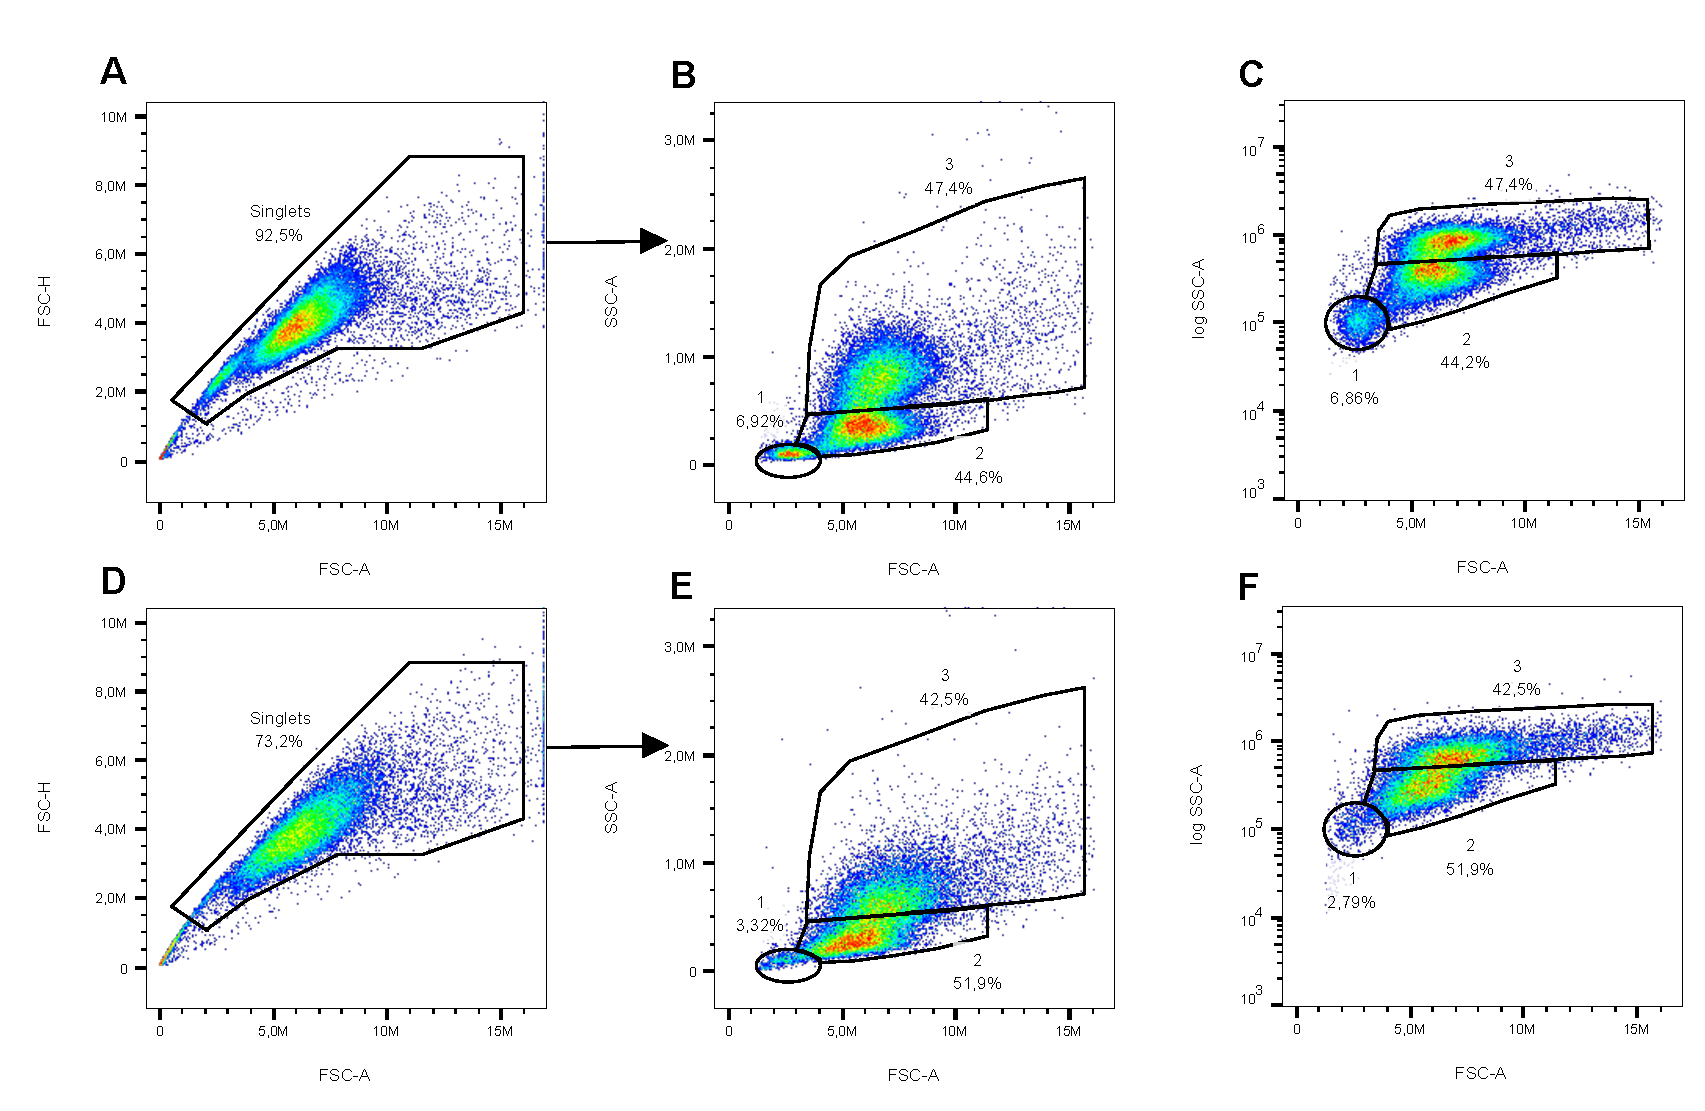
\includegraphics[width=1.0\textwidth]{figures/Gating strategy/lin to log.pdf}
    \caption{Hemocyte subpopulations distinguishable according to FSC vs. SSC \textbf{A} Bla bla bla.. Mention that the actual proportion was calculated counting 1000 hemocytes, and that the gates were adjusted to the true value.}
    \label{fig:fsc_vs_ssc}
\end{figure}

In some adult mussels, however, the basophilic and eosinophilic granulocyte subpopulations are partly overlapping with regard to internal complexity, i.e., SSC. Since the BD Accuri C6 Plus isn't equipped with adjustable laser gain settings, these subpopulations could not be separated further instrumentally. Thus, any attempts to gate on these subpopulations based solely on light scattering profiles, would in some mussels introduce considerable uncertainty into their relative proportions. [Find the proportion of mussels where they are not well separated, and report that number instead of saying "some" mussels here.]

Since eosinophilic granulocytes 

, and display higher density of granules (granularity), a bivariate plot of green fluorescence (518-548 nm) on log scale vs. SSC could accurately separate these subpopulations in about 1/10 of individuals (n=46, HMS data, data not shown), however the mean absolute error were [continue here]



\subsection{Eosinophilic granulocytes}


SD og absolute error

Hemocyte subpopulations and clusters

Light-scattering properties (optical characteristics)

[After the eosinophils had sedimented in the MAS buffer (sample M2 in sedimentation dataset) for 2 hours post-withdrawal (1:1), the percentage of eosinophils remaining in suspension were 72/1075 = 6.6976 \%. The 10k ToPro3 Calcein stained plot shows 7.91\%.]

\begin{figure}[!ht]
    \centering
    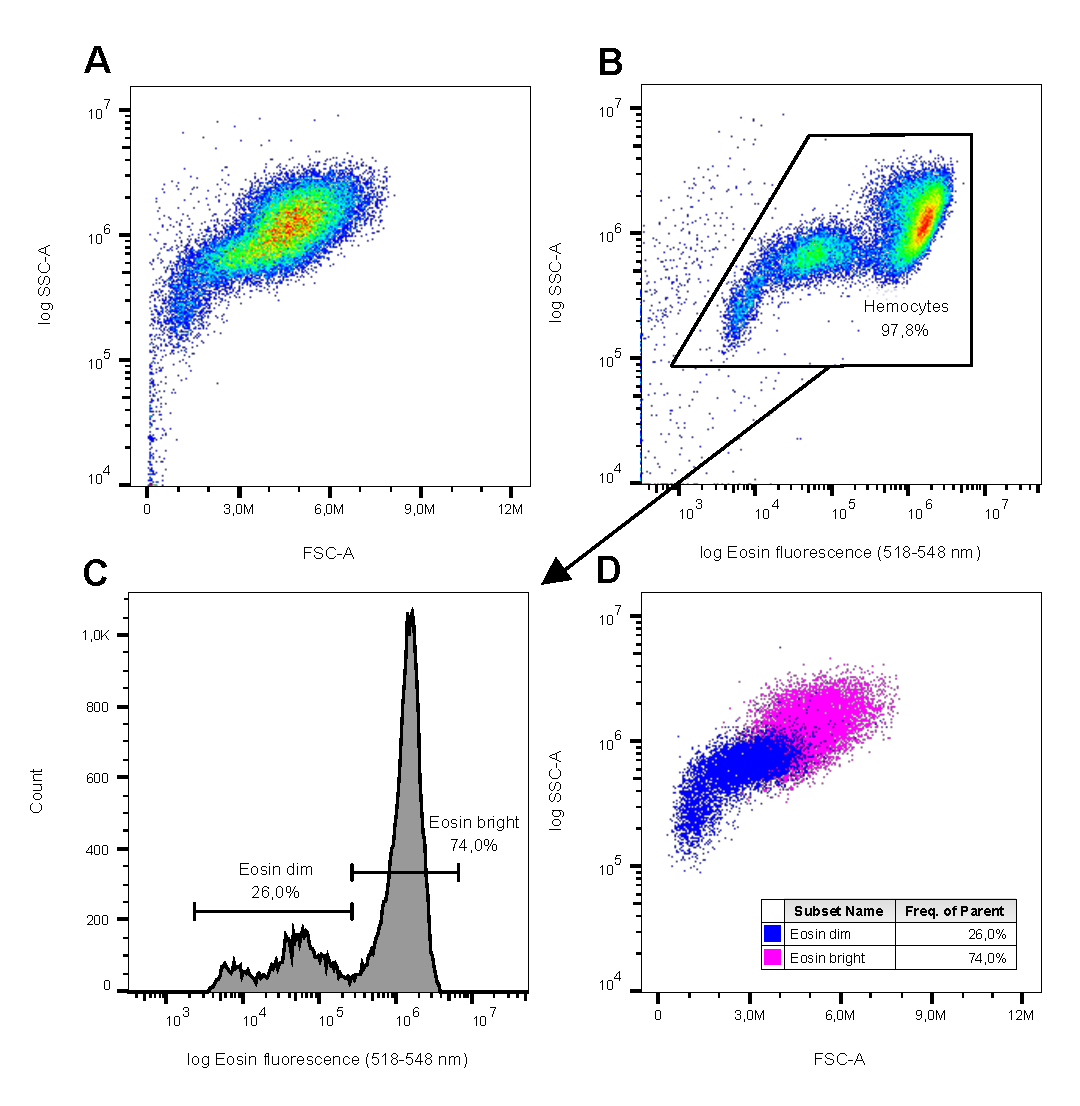
\includegraphics[width=1.0\textwidth]{figures/Eosin and Percoll exp/Pool II 0.75 per m.pdf}
    \caption{\textbf{Identification eosinophilic granulocytes. A} Representative light scatter profiles of... \textbf{B} }
    \label{fig:eosin_exp2}
\end{figure}

\begin{figure}[!ht]
    \centering
    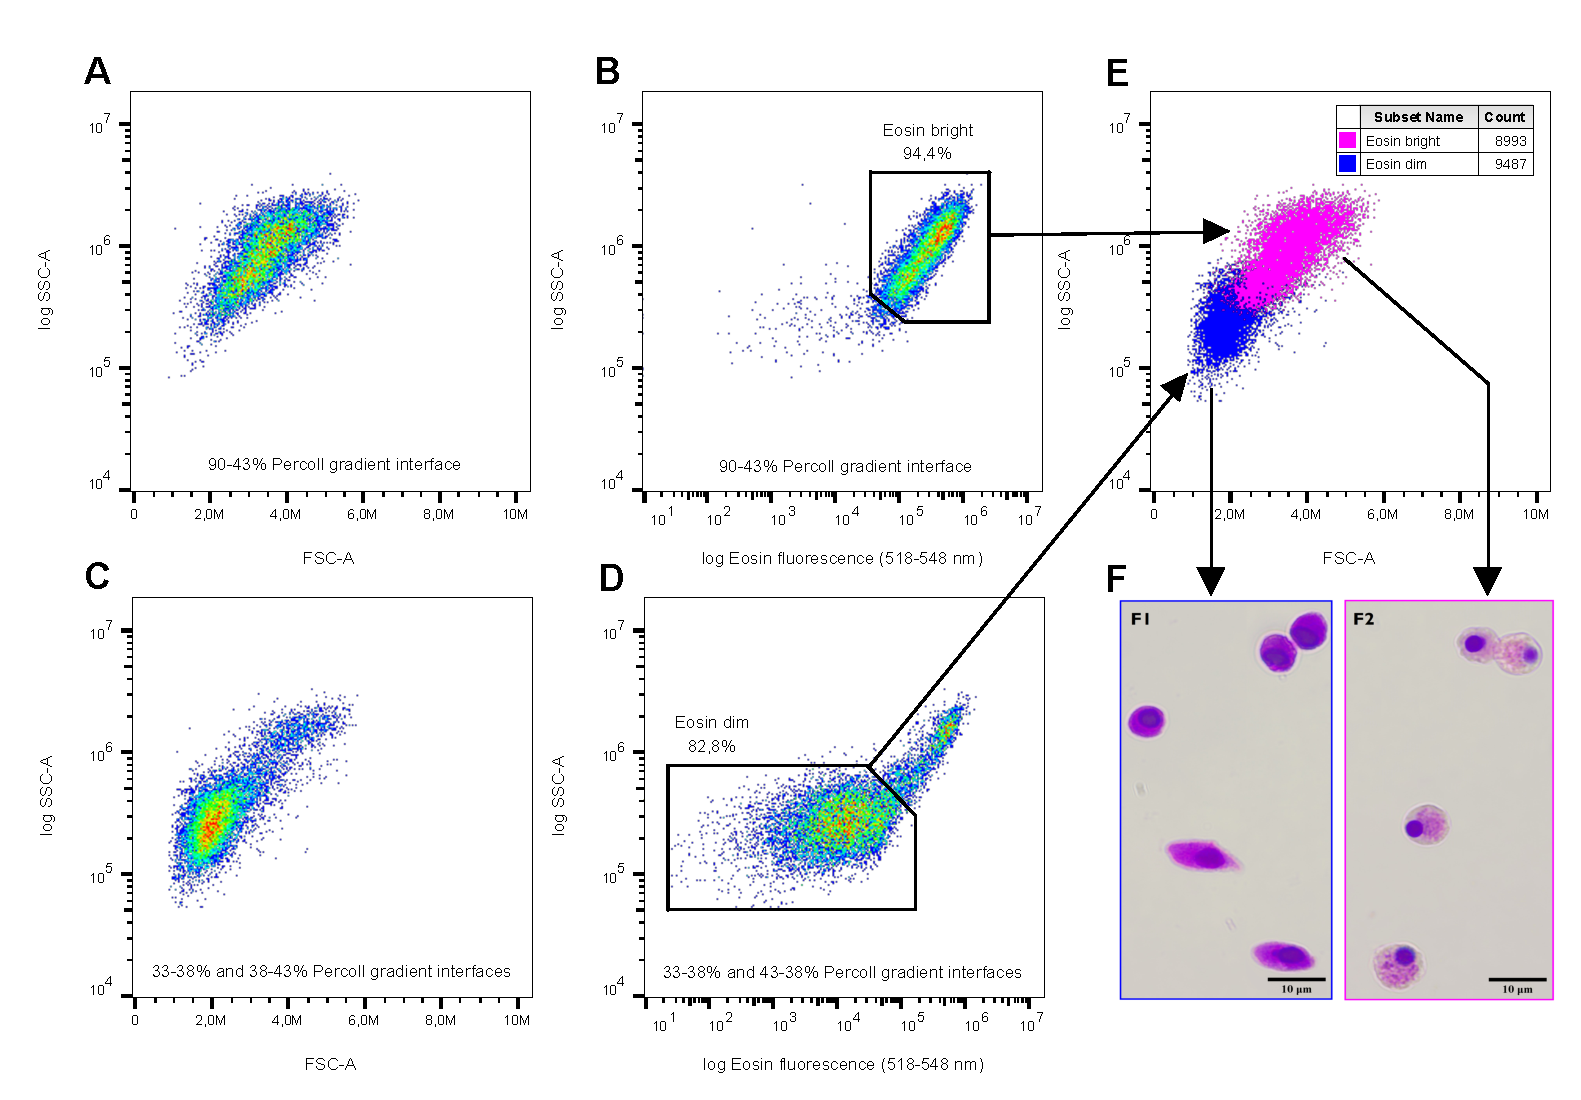
\includegraphics[width=1.0\textwidth]{figures/Eosin and Percoll exp/Percoll sep for Inkscape 2.pdf}
    \caption{\textbf{Confirmation of the light scattering profiles of eosinophilic and basophilic granulocytes pre-separated by discontinuous density centrifugation. A} Light scattering profile of the 95\% pure eosinophilic fraction that separated out on top of the 43-90\% Percoll gradient interface. \textbf{B} Bla bla bla eosin separation bla bla...}
    \label{fig:Percoll-dotplots}
\end{figure}







